\section{B\'asico}

Aqui ser\~ao apresentados alguns dos conceitos b\'asicos necess\'arios para a compreens\~ao das principais aplicaç\~oes de eletr\^onica em rob\'otica m\'ovel.

\subsection{Elementos b\'asicos}


\begin{enumerate}
\item Resistor:
	O elemento mais utilizado na confecç\~ao de circuitos eletr\^onicos, é um componente chave pois permite limitar a corrente el\'etrica que passa por elementos em s\'erie, e possibilita a aplicaç\~ao de uma tens\~ao desejada atrav\'es do conceito de divisor de tens\~ao.
		\\Por definiç\~ao \'e um componente que oferece uma oposiç\~ao \`a passagem de corrente el\'etrica, dissipando energia atrav\'es do efeito Joule.
		
\item Capacitor: 
	O capacitor \'e um elemento que armazena energia na forma de campo el\'etrico, criando uma diferença de potencial entre os seus terminais. Apesar de aparentemente possuir aplicaç\~ao apenas em circuitos em corrente alternada, \'e de extrema import\^ancia nos circuitos de corrente cont\'inua. Sua aplicaç\~ao mais utilizada \'e na filtragem dos sinais, ajudando a evitar ripples e interfer\^encias indesejadas. Nesse \^ambito pode-se citar os capacitores de desacoplamento, que geralmente ficam em paralelo com a alimentaç\~ao dos chips eletr\^onicos, e evitam variaç\~oes de tens\~ao ou interfer\^encias sobre o mesmo. Um valor t\'ipico de capacitor de desacoplamento \'e de 100nF.
	
\item Diodo:
	O diodo \'e um elemento composto de cristal semicondutor, tipicamente de germ\^anio ou sil\'icio, sendo o mais simples dos elementos semicondutores, por ser composto apenas por um cristal N e um cristal P. Suas aplicaç\~oes mais importantes est\~ao relacionadas com sua caracter\'istica de conduzir apenas quando for polarizado de forma direta, ou seja, a corrente passa apenas em um sentido pelo diodo (o que explica a sua simbologia, uma seta, que aponta para o sentido da corrente passante). Outra caracter\'istica importante \'e a queda de tens\~ao que ocorre entre os seus terminais, que \'e tipicamente de 0,7V (no cristal de sil\'icio, o mais utilizado), e que varia dependendo do material semicondutor empregado.
	\\Uma aplicação cl\'assica \'e a ponte de diodos, que permite que uma tens\~ao alternada passe a ter apenas tens\~oes positivas (faz um rebatimento dos semi-ciclos negativos no eixo x). Esse sinal pode ser então regulado e filtrado (utilizando reguladores da fam\'ilia 78XX e capacitores, por exemplo). Esse \'e o princ\'ipio de funcionamento de fontes lineares (que convertem a tens\~ao da rede em tens\~ao cont\'inua).
	
\item Transistor:
	O transistor \'e um componente eletr\^onico que revolucionou a eletr\^onica por volta dos anos 60, por apresentar uma alternativa mais compacta \`as v\'alvulas e rel\'es, al\'em de possuir uma autonomia muito maior por ter seu funcionamento baseado nos efeitos de campo do seu material semi-condutor. Pode ser utilizado como chave (deve estar trabalhando na zona de saturaç\~ao) ou como amplificador (deve estar trabalhando na zona linear).
\end{enumerate}

\subsection{Aplicaç\~oes em Rob\'otica M\'ovel}

A eletr\^onica se mostra de extrema import\^ancia no \^ambito da rob\'otica m\'ovel, estando presente em praticamente todos os m\'odulos que juntos comp\~oe um rob\^o.
Logo abaixo est\~ao listados alguns exemplos de aplicaç\~ao de elementos e circuitos eletr\^onicos em um rob\^o.
\\Primeiramente haver\'a uma abordagem sobre sensores e atuadores, que basicamente s\~ao elementos que possibilitam todo tipo de interaç\~ao do rob\^o com o ambiente, cada vez mais necess\'aria \`a medidada em que a ``intelig\^encia" dos rob\^os aumenta. Logo ap\'os ser\~ao abordados os microcontroladores e computadores que s\~ao cada vez mais embarcados nos rob\^os (e em tudo o que se possa pensar no mundo), e s\~ao como um c\'erebro do rob\^o (talvez n\~ao seja o termo mais adequado, j\'a que com a diminuiç\~ao nos preços de microcontroladores o processamento de dados est\'a sendo mais distribuido em processadores pr\'oximos aos diversos elementos do rob\^o).

\begin{enumerate}
\item Sensores:
	Sensores s\~ao dispositivos sens\'iveis \`a fen\^omenos f\'isicos ou qu\'imicos, transformando-os em uma grandeza mensur\'avel. Nos seres vivos notamos a existência de diversos sensores, permitindo a interaç\~ao do organismo com o meio exterior (a vis\~ao, por exemplo utiliza sensores para interpretar as cores atrav\'es da frequ\^encia dos f\'otons de luz, os cones, e outros sensores para a luminosidade atrav\'es da quantidade de f\'otons de luz, os bastonetes).
	Quando o sensor converte esse fen\^omeno em um sinal el\'etrico (de tens\~ao ou corrente), ele \'e chamado de transdutor. Em suma, todos os sensores utilizados em rob\'otica m\'ovel s\~ao transdutores, logo necessitam de um circuito eletr\^onico para interpretar a grandeza medida, podendo ser apenas um comparador anal\'ogico utilizando amplificadores operacinais ou um circuito microcontrolado para tratar o sinal de sa\'ida do sensor. Atualmente a segunda opç\~ao, microcontrolada \'e amplamente utilizada, devido \`a reduç\~ao dos preços dos microcontroladores, e \`as vantagens relacionadas, como a transmiss\~ao de dados de forma digital (sinais alan\'ogicos s\~ao mais sucet\'iveis a ru\'idos e interfer\^encias).
	Uma tend\^encia j\'a amplamente aplicada \'e a de sensores inteligentes, que s\~ao sensores com um microcontrolador embarcado, agregando funcionalidades interessantes, como a digitalizaç\~ao dos dados, e possibilitando outras, nem sempre utilizadas, como a calibraç\~ao do sensor, supervis\~ao de valores limite, compactaç\~ao de dados e eliminaç\~ao de redund\^ancias, filtragem digital do sinal, correç\~ao autom\'atica de erros sistem\'aticos (não linearidade, dependências de temperatura, etc).\cite{apostilaStemmer}
	
\item Atuadores:
	\begin{quote}
	Atuador é um elemento que produz movimento, atendendo a comandos que podem ser manuais, elétricos ou mecânicos. Como exemplo, pode-se citar atuadores de movimento induzido por cilindros pneumáticos (pneumática) ou cilindros hidráulicos (Hidráulica) e motores (dispositivos rotativos com acionamento de diversas naturezas).
	\\- http://pt.wikipedia.org/wiki/Atuador
	\end{quote}
	Dentre estes atuadores citados, os que envolvem diretamente conceitos e circuitos eletr\^onicos s\~ao os motores, do tipo el\'etrico, sendo tamb\'em os mais utilizados no \^ambito da rob\'otica m\'ovel.
	
\item Microcontroladores:
	Um microcontrolador \'e um pequeno computador com diversos perif\'ericos dentro de um \'unico chip. Enquanto um microprocessador (como os que encontramos dentro dos PC's) apresenta apenas a ULA (unidade de l\'ogica aritm\'etica) e registradores, o microcontrolador apresenta mem\'orias EEPROM e RAM, conversores anal\'ogico-digital, interfaces de entrada-sa\'ida, clock interno e outros elementos. Obviamente por apresentar v\'arios elementos dentro do mesmo chip, eles n\~ao s\~ao t\~ao eficientes quanto um microprocessador, e trabalham em frequ\^encia muito mais baixa, na ordem de MHz, por\'em s\~ao extremamente pr\'aticos por n\~ao necessitarem de perif\'ericos externos para funcionar, serem de baixo custo e permitirem a gravaç\~ao dos programas diretamente no chip.
	\\Existem microcontroladores com diversas capacidades de processamento, o que tamb\'em influencia seu preço. Primeiramente temos os processadores de 8 bits, utilizados em aplicaç\~oes que n\~ao exigem muito poder de processamento, como o tratamento de um sinal anal\'ogico (de um sensor, por exemplo) ou o controle de um motor. Nessa categoria os microcontroladores mais populares s\~ao os PICs da fam\'ilia 16F e 18F, que s\~ao microcontroladores de arquitetura RISC (reduced instruction set computing), que funcionam em frequências de cerca de 4MHz a 20Mhz e possuem diversos perif\'ericos como conversores AD, protocolos de comunicaç\~ao implementados em hardware (USART, I2C, SPI e no caso de alguns 18Fs, USB), PWM (pulse width modulation), etc.
	
\item Computadores:


\end{enumerate}



\section{Placa de Circuito Impresso}
Nesa seç\~ao ser\'a abordado um tema de extrema import\^ancia para a eletr\^onica, que \'e relativo \`as placas de circuito impresso, que a partir de agora ser\~ao chamadas de PCB, do ingl\^es 'printed circuit board'. Saber confeccionar uma PCB significa transformar um circuito desenhado no papel em realidade, e envolve uma vasta gama de conhecimento, que ser\'a (\`a medida do poss\'ivel) condensado e resumido aqui.

\subsection{O que \'e?}

A PCB \'e uma placa, geralmente de fenolite, podendo ser tamb\'em de fibra de vidro ou de poli\'ester, com uma fina camada de cobre que \'e corro\'ida de forma a criar caminhos para conectar eletricamente componentes eletr\^onicos (chamados de trilhas), formando assim o circuito eletr\^onico desejado. A PCB foi criada para substituir a ponte de terminais, que era utilizada anteriormente, e que impedia a implementaç\~ao de circuitos mais complexos, devido aos diversos problemas de interfer\^encia e pela pr\'opria disposiç\~ao f\'isica dos componentes, que muitas vezes beiravam o caos. Outro problema encontrado nessa t\'ecnica arcaica era a produç\~ao em s\'erie dos circuitos, um processo dif\'icil de ser mecanizado e bastante meticuloso.
\\Inicialmente o desenho do circuito na placa (layout) era feito manualmente, com o aux\'ilio de r\'eguas que continham os moldes dos principais componentes utilizados, e as trilhas eram desenhadas \`a m\~ao com uma caneta permanente ou com o aux\'ilio de fitas adesivas. Obviamente hoje em dia existem softwares de computador, chamados CADs (computer aidded design) que possibilitam esse projeto. Ap\'os possuir o  layout pronto, pode-se mandar produzir as placas em alguma empresa especializada, que utiliza ferramentas avançadas possibilitando placas complexas e com componentes pequenos, ou pode-se utilizar m\'etodos artesanais para produzir essa placa, que acaba limitando a complexidade do projeto, por\'em \'e suficiente para v\'arias aplicaç\~oes interessantes.

\subsection{Elementos b\'asicos}

Aqui ser\~ao apresentados alguns conceitos e termos utilizados de forma a possibilitar o entendimento dos t\'opicos subsequentes.

\begin{enumerate}

\item Trilha: As trilhas s\~ao `caminhos' de cobre que fazem as ligaç\~oes el\'etricas necess\'arias nas placas. Sua largura est\'a relacionada com a corrente que deve passar por ela, devendo ser gradativamente mais larga ao se esperar maiores valores de corrente, e esta deve ser uma preocupaç\~ao do respons\'avel pelo layout. O risco de subdimensionar a largura da trilha \'e de, quando uma corrente muito grande passar, o cobre esquentar muito e descolar da placa, podendo at\'e mesmo fundir e romper. Isso ocorre pois a resist\^encia el\'etrica associada \'e inversamente proporcional \`a largura da trilha, e pela lei de Joule o calor dissipado \'e maior com o aumento da resist\^encia (mantendo-se a corrente passante).

\item Camadas (layers): As camadas de cobre presente em uma PCB s\~ao chamadas layers. As placas mais simples possuem apenas uma camada de cobre e s\~ao chamadas single-layer, sendo as mais utilizadas por hobbistas que utilizam processos caseiros de fabricaç\~ao das placas. Quando a placa possui duas camadas de cobre \'e chamada de dual-layer, e pode tamb\'em ser confeccionada com m\'etodos caseiros, por\'em com mais dificuldade, pois deve-se projetar o layout para os dois lados e depois sincroniz\'a-los para que os furos coincidam. Quando a placa possui mais de duas camadas \'e chamada multi-layer, e s\'o pode ser feita atrav\'es de processos industriais, com a utilizaç\~ao de materiais e m\'aquinas espec\'ificas para tal.

\item Componentes Through-Hole: S\~ao componentes que se utilizam de pinos met\'alicos que devem atravessar a placa atrav\'es de um furo, podendo ser metalizado ou n\~ao, sendo soldados no lado oposto ao componente.

\item Componentes SMD: Os componentes SMD (surface mount devices, ou dispositivos de montagem superficial), s\~ao componentes que s\~ao soldados diretamente sobre a face de cobre da PCB, sem utilizar furos para sua fixaç\~ao mec\^anica.

\item Ilhas (pads): As ilhas s\~ao superf\'icies de cobre onde os componentes s\~ao soldados. Geralmente s\~ao redondas para componentes through-hole e quadradas para os SMD.



\end{enumerate}

\subsection{CADs}

Os CADs (computer aidded design) s\~ao softwares que auxiliam no projeto e desenho t\'ecnico nas mais diversas \'areas, como no projeto de construç\~oes, de peças mec\^anicas e de PCB's, substituindo a necessidade de utilizar os processos manuais para o desenho das plantas, vistas e layouts, respectivamente. Os principais softwares do mercado oferecem ferramentas que facilitam o processo, reduzindo drasticamente o tempo de projeto e de eventuais reparos em um design j\'a existente.


\section{Softwares}
Nesta seç\~ao ser\~ao apresentados os principais softwares utilizados em aplicaç\~oes para eletr\^onica. Tais softwares s\~ao extremamente \'uteis para a realizaç\~ao de um projeto, principalmente para o projeto de placas de circuito. Esses softwares s\~ao chamados CAD's (computer aided design, ou desenho assistido em computador em portugu\^es) e geralmente permitem o projeto tanto do esquem\'atico quanto do layout da placa, tamb\'em chamado PCB (printed circuit board, ou placa de circuito impresso em portugu\^es) design. Outros softwares s\~ao utilizados pra realizar a simulaç\~ao de circuitos eletr\^onicos, acabando com a necessidade de realizar certos c\'alculos manualmente, e em alguns casos agregando aspectos pr\'aticos dos elementos, como indut\^ancias, capacit\^ancias e resist\^encias que n\~ao existem nos modelos ideais. Alguns softwares agregam todas essas funcionalidades, como \'e o caso do Proteus.
Abaixo est\~ao listados alguns dos principais softwares utilizados, com uma descriç\~ao de cada um.

\subsection{Proteus}
Desenvolvido pela empresa inglesa Labcenter Electronics, o Proteus \'e provavelmente o software mais utilizado por hobistas ao redor do mundo, principalmente pela possibilidade de simulaç\~ao de diversos microcontroladores, como os PICs da microchip e Atmegas da Atmel, além de v\'arios ARMs.
O Proteus Design Suite \'e dividido em dois softwares, o ISIS e o ARES. O primeiro \'e o programa respons\'avel pelo desenho dos esquem\'aticos, al\'em das simulaç\~oes de circuitos eletr\^onicos.

\begin{figure}[htb]
\center
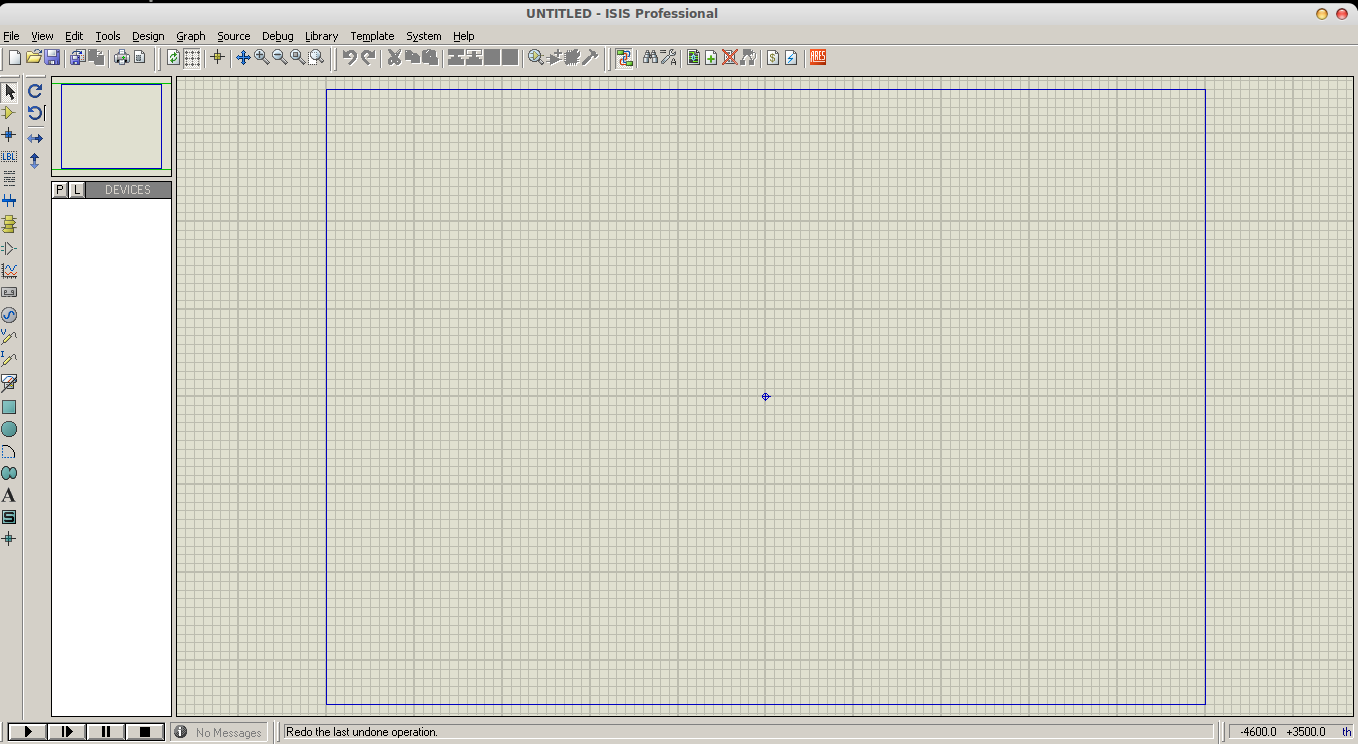
\includegraphics[width=1\textwidth]{./include/chapters/sections/hard/section1/img/Isis_homescreen.png}
\caption{Tela inicial do ISIS}
\label{IsisHome}
\end{figure}

J\'a o Ares \'e utilizado para a criaç\~ao do layout da PCB. Possui um auto-router, que roteia as trilhas automaticamente, utilizando as conex\~oes do esquem\'atico criado no ISIS. Outra funç\~ao interessante do Ares \'e a possibilidade de uma visualizaç\~ao em 3D da placa em desenvolvimento, desde que os componentes utilizados possuam um modelo em 3D.

\begin{figure}[htb]
\center
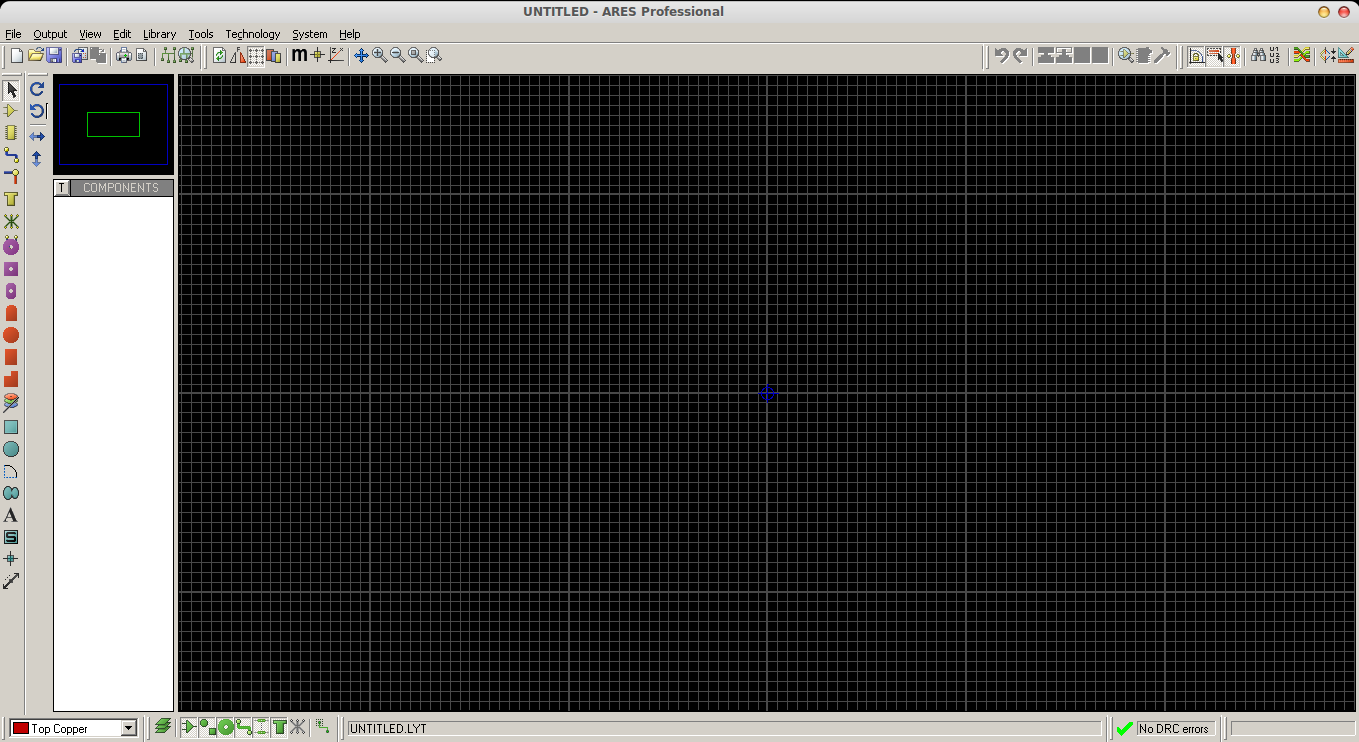
\includegraphics[width=1\textwidth]{./include/chapters/sections/hard/section1/img/Ares_homescreen.png}
\caption{Tela inicial do Ares}
\label{AresHome}
\end{figure}


\subsection{Eagle}
O Eagle (sigla de Easily Applicable Graphical Layout Editor) \'e um CAD desenvolvido pela empresa CadSoft Computer com suas primeiras ediç\~oes jur\'assicas feitas para rodar no DOS, ainda como um aplicativo de 16 bits. Atualmente possui vers\~oes para Windows, Linux e Mac OS. Possui um editor para desenhar os esquem\'aticos de cirucitos eletr\^onicos, um editor para criar o layout das placas de circuito impresso, auto-router al\'em de diversas outras ferramentas.
\\Apesar de ser um programa pago, \'e o software mais utilizado entre usu\'arios adeptos ao open source, pois sua vers\~ao freeware possui apenas uma limitaç\~ao quanto ao tamanho do projeto (que n\~ao \'e problema em aplicaç\~oes usuais), mas principalmente por possuir uma gigantesca biblioteca com os footprints dos mais variados componentes na rede, constru\'ida pelos in\'umeros hobistas que utilizam o programa.
\\\'E importante ressaltar que o Eagle \'e um programa que possui uma curva de aprendizado grande, por\'em por possuir muitos adeptos \'e f\'acil encontrar material na internet que possa ajudar a utiliz\'a-lo.

\begin{figure}[htb]
\center
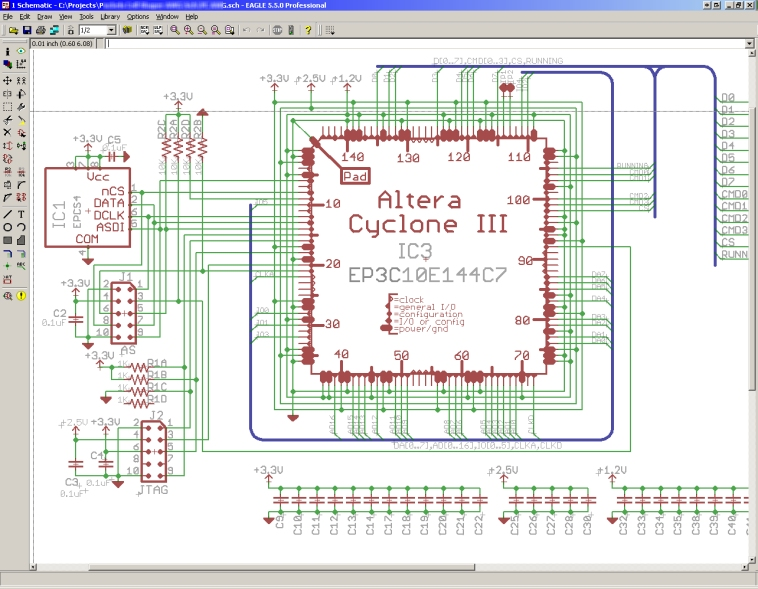
\includegraphics[width=1\textwidth]{./include/chapters/sections/hard/section1/img/Eagle_schem.jpg}
\caption{Editor de esquem\'aticos do Eagle}
\label{Eagle_schem}
\end{figure}

\begin{figure}[htb]
\center
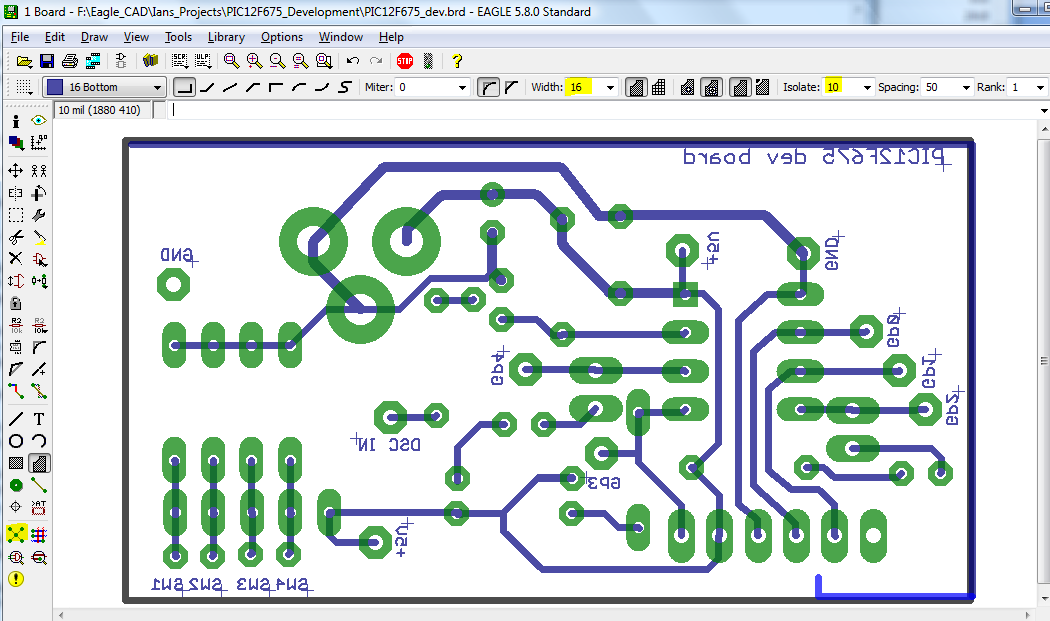
\includegraphics[width=1\textwidth]{./include/chapters/sections/hard/section1/img/Eagle_layout.png}
\caption{Editor de layout do Eagle}
\label{Eagle_layout}
\end{figure}

\subsection{Altium Designer}
Possivelmene um dos mais completos programas para desenvolvimente de projetos eletr\^onicos, sendo desenvolvido pela empresa Australiana Altium Limited, \'e baseado  no famoso Protel, um software muito utilizado at\'e o começo dos anos 2000's. Possui a mais variada mir\'iade de funcionalidades e ferramentas para o desenvolvimento de placas de circuito impresso e FPGA's. \'E recomendado para projetos complexos, lidando bem com placas com m\'ultiplas camadas e componentes SMD. Possui um poderoso visualizador 3D (na verdade foi o primeiro software a apresentar essa ferramenta, em 2007), preciso e muito \'util para averiguar corriqueiros conflitos mec\^anicos que possam ocorrer no roteamento da placa. Software utilizado por diversas empresas que produzem placas com n\'ivel de complexidade elevado, interessante para quem deseja ter contato com um software de n\'ivel profissional.

\subsection{Psim}
